\documentclass[10pt,twocolumn,letterpaper]{article}

\usepackage{cvpr}
\usepackage{times}
\usepackage{epsfig}
\usepackage{graphicx}
\usepackage{amsmath}
\usepackage{amssymb}

% Include other packages here, before hyperref.

% If you comment hyperref and then uncomment it, you should delete
% egpaper.aux before re-running latex.  (Or just hit 'q' on the first latex
% run, let it finish, and you should be clear).
%\usepackage[pagebackref=true,breaklinks=true,letterpaper=true,colorlinks,bookmarks=false]{hyperref}

\cvprfinalcopy % *** Uncomment this line for the final submission

\def\cvprPaperID{****} % *** Enter the 3DV Paper ID here
\def\httilde{\mbox{\tt\raisebox{-.5ex}{\symbol{126}}}}

% Pages are numbered in submission mode, and unnumbered in camera-ready
%\ifcvprfinal\pagestyle{empty}\fi
\setcounter{page}{1}
\begin{document}

%%%%%%%%% TITLE
\title{Image Reconstruction from DVS\\ The constant battle agains MATLAB\\ Student Project Report}

\author{Samuel Bryner\\
ETH Zurich\\
%Institution1 address\\
{\tt\small firstauthor@i1.org}
% For a paper whose authors are all at the same institution,
% omit the following lines up until the closing ``}''.
% Additional authors and addresses can be added with ``\and'',
% just like the second author.
% To save space, use either the email address or home page, not both
\and
Marcel Geppert\\
ETH Zurich\\
%First line of institution2 address\\
{\tt\small secondauthor@i2.org}
}

\maketitle
%\thispagestyle{empty}

%%%%%%%%% ABSTRACT
\begin{abstract}

// TODO - insert abstract

\end{abstract}

%%%%%%%%% BODY TEXT
\section{Introduction}

// TODO - insert introduction here

%-------------------------------------------------------------------------
\section{Related Work}

// TODO - insert related work here

-Kim \etal\\
-Scaramuzza\\
-\cite{lpd08dvs}\\
-vSLAM?\\

\section{Dynamic Vision Sensors}

A Dynamic Vision Sensor (DVS) \cite{lpd08dvs}, also known as an event camera,
is a new kind of camera. In contrast to a standard camera it does not output a
complete image of the scene, but a series of events. An event is generated when
the sensed brightness of a pixel changes more than a certain threshold. This
happens for each pixel completely independent from all the others.

A DVS has several advantages compared to standard cameras. Since there is no
need to gather data from all pixels to generate an image, events can be sent
with an extremely low latency of $15 \mu s$ or less \cite{brandli14davis, lpd08dvs} and
with microsecond timestamps.  For the same reason, there is practically no
motion blur in the DVS signal.  Another benefit of independent pixels is the
very high dynamic range.  Saturation, blooming or smearing as observed when a
bright light source is captured with a standard camera is basically
nonexistent. Finally, due to the reduction of the camera signal to changes and
the resulting elimination of redundant temporal information, the signal
bandwidth is much smaller than with a standard camera.
All these features make the DVS a very desirable sensor for motion tracking,
especially for mobile robots where the data has to be analyzed on constrained
hardware.

However, there are currently several caveats: First of all, currently available
DVS (DVS128 \cite{lpd08dvs}, DAVIS \cite{brandli14davis}) have a very limited
resolution of $128 \times 128$ or $240 \times 180$ pixels, respectively. This
obviously limits the spacial accuracy of the sensed data, but it is likely to
be a simple matter of time until sensors with a higher resolution are
developed. A more important point is that the computer vision algorithms that
have been developed during the last decades either cannot be used at all or
have to be adapted to the new data representation.


\section{Our Work}

// TODO - insert section to explain what we did here

-implemented paper (kim) in matlab\\
-some simplifications\\
	-use particle filter directly with euler angles (ignore corner cases)\\
	-start with first fov in map\\
	
\section{Core Algorithm}

// TODO - insert overview over core algorithm

\subsection{Rotation Tracking}

// TODO - insert section about tracking

\subsection{Scene Reconstruction}

We use Kalman Filters to reconstruct the grayscale image from the noisy DVS signal. For each pixel in the output image there is a Kalman Filter that keeps track of the color gradient at the pixel position. The input to the Kalman Filter is the event frequency on a line along the current pixel movement. Hereby it is assumed that the pixel's movement was constant since the last event it triggered. While this is obviously not true all the time, it is a good approximation due to the high rate of events. Note that the pixel movement is not necessarily parallel to the camera movement, e.g. if the camera is rotating around its z-axis.
The pixel movement is computed with the same formulas as used in the simulationand the map lookup during tracking. Given a camera orientation, the orientation of the ray through the pixel and the camera's focal point is computed. This is then mapped to a pixel in the output image. While we use the exact position in the output image to compute the pixel movement,  we do not, however, interpolate between several pixels when writing the signal to the map, but simply round the position in the output image th the closest pixel. Since we do not write the signal directly but use Kalman Filters to reduce the noise, this simplification greatly reduces the complexity of the algorithm compared to dividing the signals between several filters.
The exact formulas used for the Kalman Filters can be seen in \cite{kim2014simultaneous}.
In the current state of our program, we assume that the camera's initial field of view is already known and included in the map. With this assumption we do not have to deal with a special initialization procedure but can immediately start with the standard iteration while being relatively sure that the camera movement is tracked correctly.


\section{Problems}

// TODO - insert section about problems

-map initialization\\
-runtime\\
$\rightarrow$ couldn't test with camera\\
-MATLAB\\


\section{Experiments}

// TODO - insert section about experiments

-initialization\\
	-integrate whie removing shutter\\
	-integrate over short interval\\
	
-camera calibration\\

\subsection{Camera Simulation}

// TODO insert section to explain camera simulation

-use image as input\\
-assume 360 deg view\\
-compute camera fov for given orientation\\
-move camera over scene\\
-sum up differences between patches\\
-problem: discrete\\
	$\rightarrow$ use tiny steps\\
		$\rightarrow$ slow\\

\section{Results}

TODO: write some text here. Conclusion and stuff.

- influence of the various parameters
- code too slow for realtime, but not optimized at all
- using Matlab for more than just a few hacked scripts: bad idea

\begin{figure}
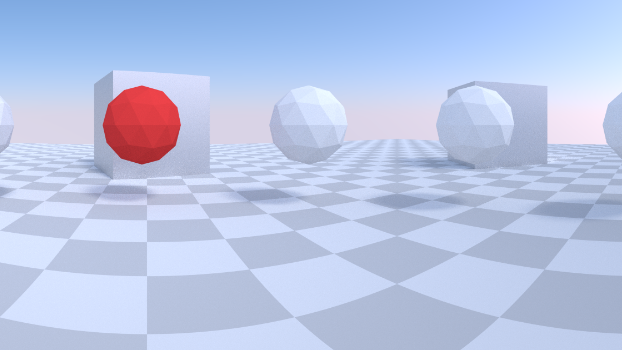
\includegraphics[width=\columnwidth]{images/zigzag_input.png}
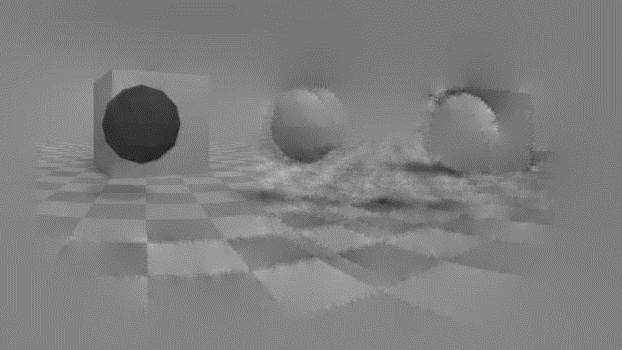
\includegraphics[width=\columnwidth]{images/zigzag_reconstruction.png}
\caption{A part of the input scene (top) and its reconstruction,
moving the camera in a large triangle waveform pattern to the right.
The area around the leftmost ball in the scene was used to initialize
the map as described in section \ref{sec:core_algorithm}.}
\label{fig:zigzag_reconstruction}
\end{figure}



{\small
\bibliographystyle{ieee}
\bibliography{references}
}

\end{document}
